%--------------------------------------------------------------- %
\documentclass[SPC-MASTER.tex]{subfiles}
\begin{document}
	\Large
\section{Multivariate Control Charts}
{\large
%MSQC book Part 2
\begin{itemize}
\item With the enhancements in data acquisition systems it is usual to deal with processes
with more than one correlated quality characteristic to be monitored. 
\item A common
practice is to control the stability of the process using univariate control charts. 
\item This
practice increases the probability of false alarm of special cause of variation.
\item Therefore, the analysis should be performed through a multivariate approach;
that is, the variables must be analyzed together, not independently.
\end{itemize}

\subsection{Multivariate Control Charts}
% http://www.jmp.com/support/help/Multivariate_Control_Charts.shtml
{\large\begin{itemize}
\item Multivariate control charts monitor multiple process characteristics. Independent variables can be charted individually, but if the variables are correlated, a multivariate chart is needed to determine whether the process is in control. 
\item Multivariate control charts can detect shifts in the mean or the relationship between several related variables.
\item 
The multivariate control chart plots Hotelling’s T2 statistic. The calculation for the control limit differs based on whether targets have been specified.
\end{itemize}}

\subsection{The MSQC package}

In his book, Edgar Santos-Fernandez present the multivariate normal distribution, the data structure
of the multivariate problems dealt in this book, the mult.chart function that allows
the computation in R, and the most used multivariate control charts:
}
\begin{itemize}
\item The control ellipsoid or w2 control chart
\item The T2 or Hotelling chart
\item The Multivariate Exponentially Weighted Moving Average (MEWMA) chart
\item The Multivariate Cumulative Sum (MCUSUM) chart
\item The chart based on Principal Components Analysis (PCA)
\end{itemize} 

\subsection{The \texttt{mult.chart} Function}
The performing of the multivariate control chart in R can be carried out with the
function mult.chart which is a general function that allows to compute the most
accepted and diversified continuous multivariate chart such as

\begin{itemize} 
\item $\chi^2$
\item Hotelling $T^2$
\item MEWMA
\item MCUSUM according to Crosier (1988)
\item MCUSUM by Pignatiello and Runger (1990)
\end{itemize}
Finally the function \texttt{mult.chart} returns:

\begin{itemize} 
\item The T2 statistics
\item The Upper Control Limit (UCL)
\item The sample covariance matrix (S)
\item The mean vector (Xmv)
\item And if any point falls outside of the UCL and its decomposition
\end{itemize}

\begin{framed}
\begin{verbatim}
mult.chart(dowel1, type = "chi", alpha = 0.05)
\end{verbatim}
\end{framed}

\subsection{T2 control chart}
\large
The origin of the T2 control chart dates back to the pioneer works of Harold Hotelling
who applied this method to the bombsight problem in Second World War. The
Hotelling (1947) procedure has become without doubt the most applied in multivariate
process control and it is the multivariate analogous of the Shewhart control chart.
For that reason, it is also known as multivariate Shewhart control chart.
\begin{framed}
\begin{verbatim}
data("carbon1")
mult.chart(type = "t2", carbon1)
mult.chart(type = "t2", carbon1)$t2
\end{verbatim}
\end{framed}
\newpage

%--------------------------------------------------------------- %
\newpage
\subsection{\texttt{mqcc} Example}
\begin{framed}
\begin{verbatim}
# library(mqcc)
# Ryan (2000, Table 9.2) data with p = 2 variables, 
#  m = 20 samples, n = 4 sample size:

X1 = matrix(c(72, 56, 55, 44, 97, 83, 47, 88, 57, 26, 46,
49, 71, 71, 67, 55, 49, 72, 61, 35, 84, 87, 73, 80, 26, 89, 66,
50, 47, 39, 27, 62, 63, 58, 69, 63, 51, 80, 74, 38, 79, 33, 22,
54, 48, 91, 53, 84, 41, 52, 63, 78, 82, 69, 70, 72, 55, 61, 62,
41, 49, 42, 60, 74, 58, 62, 58, 69, 46, 48, 34, 87, 55, 70, 94,
49, 76, 59, 57, 46), ncol = 4)

X2 = matrix(c(23, 14, 13, 9, 36, 30, 12, 31, 14, 7, 10,
11, 22, 21, 18, 15, 13, 22, 19, 10, 30, 31, 22, 28, 10, 35, 18,
11, 10, 11, 8, 20, 16, 19, 19, 16, 14, 28, 20, 11, 28, 8, 6,
15, 14, 36, 14, 30, 8, 35, 19, 27, 31, 17, 18, 20, 16, 18, 16,
13, 10, 9, 16, 25, 15, 18, 16, 19, 10, 30, 9, 31, 15, 20, 35,
12, 26, 17, 14, 16), ncol = 4)

X = list(X1 = X1, X2 = X2)
q = mqcc(X, type = "T2")
summary(q)
\end{verbatim}
\end{framed}
\begin{figure}[h!]
\centering
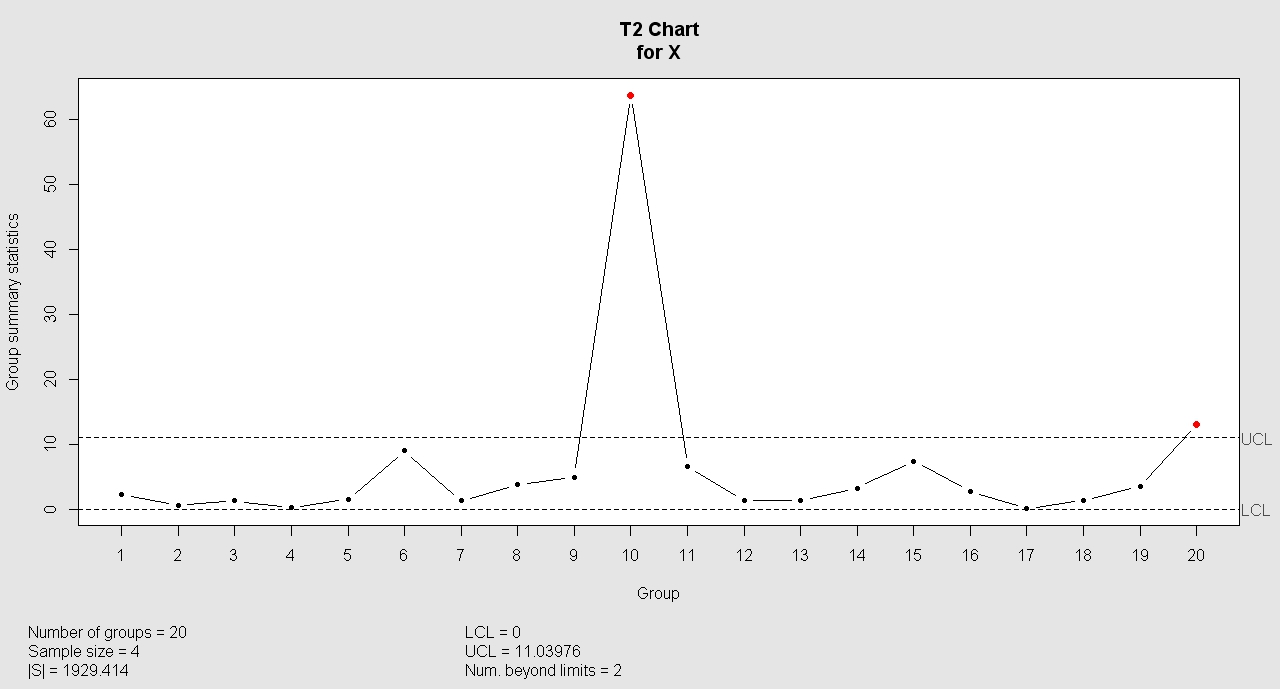
\includegraphics[width=0.9\linewidth]{images/mqccplot1}
\caption{}
\label{fig:mqccplot1}
\end{figure}
\newpage
\begin{verbatim}
Call:
mqcc(data = X, type = "T2")

T2 chart for X 

Summary of group statistics:
   Min. 1st Qu.  Median    Mean 3rd Qu.    Max. 
 0.1243  1.3250  2.5030  6.4700  5.3490 63.7600 

Number of variables:  2
Number of groups:  20
Group sample size:  4

Center: 
     X1      X2 
60.3750 18.4875 

Covariance matrix:
         X1        X2
X1 222.0333 103.11667
X2 103.1167  56.57917
|S|:  1929.414 

Control limits:
 LCL      UCL
   0 11.03976

\end{verbatim}

%\subsection{Confidence Region}
%a confidence region is a multi-dimensional generalization of a confidence interval. It is a set of points in an n-dimensional space, often represented as an ellipsoid around a point which is an estimated solution to a problem, although other shapes can occur.
%
%The confidence region is calculated in such a way that if a set of measurements were repeated many times and a confidence region calculated in the same way on each set of measurements, then a certain percentage of the time, on average, (e.g. 95%) the confidence region would include the point representing the "true" values of the set of variables being estimated. However, unless certain assumptions about prior probabilities are made, it does not mean, when one confidence region has been calculated, that there is a 95% probability that the "true" values lie inside the region, since we do not assume any particular probability distribution of the "true" values and we may or may not have other information about where they are likely to lie.
\newpage
\end{document}